\documentclass[11pt,a4paper]{article}

% ── Packages ──────────────────────────────────────────────────────────────
\usepackage[utf8]{inputenc}
\usepackage[T1]{fontenc}
\usepackage{lmodern}
\usepackage[margin=1in]{geometry}
\usepackage{graphicx}
\usepackage{booktabs}
\usepackage{hyperref}
\usepackage{xcolor}
\usepackage{caption}
\usepackage{float}
\usepackage{enumitem}
\usepackage{multirow}
\usepackage{amsmath}
\usepackage{amssymb}
\usepackage{listings}
\usepackage{tikz}
\usetikzlibrary{arrows.meta, positioning, shapes.geometric}

% ── Metadata ──────────────────────────────────────────────────────────────
\hypersetup{
    colorlinks=true,
    linkcolor=blue,
    citecolor=blue,
    urlcolor=blue
}

\lstset{
    basicstyle=\ttfamily\footnotesize,
    breaklines=true,
    frame=single,
    backgroundcolor=\color{gray!5}
}

\pagestyle{plain}

% ── Title ─────────────────────────────────────────────────────────────────
\title{\textbf{End-to-End MLOps Pipeline for Short-Term Solar Irradiance Forecasting}\\[5pt]
\large Wolf Point, Montana  --  Local Minikube Cluster Deployment}
\author{Kevin Christian Eriksson \and Max Sebastian Segerkrantz \and Lisell Aare}
\date{\today}

\begin{document}
\maketitle

% ── Abstract ──────────────────────────────────────────────────────────────
\begin{abstract}
This report presents a reproducible end-to-end MLOps pipeline for short-term solar irradiance forecasting at a fixed site in Wolf Point, Montana. The system ingests Solcast historical data at 15-minute resolution (2007--present), engineers time-series features, trains three competing models (smart persistence baseline, XGBoost, and LSTM), and deploys the best-performing model behind a FastAPI serving endpoint on a local minikube Kubernetes cluster. A closed-loop monitoring system -- comprising Prometheus, Grafana, and Alertmanager -- tracks prediction drift and skill degradation, automatically triggering retraining via a Kubeflow Pipelines webhook. The deliverable is the pipeline itself, not merely the trained model: every deployed artifact is traceable to its exact Git commit and DVC feature hash.
\end{abstract}

% ── 1. Introduction ───────────────────────────────────────────────────────
\section{Introduction}

Accurate short-term solar irradiance forecasting is critical for grid integration of photovoltaic generation, energy trading, and demand-side management. However, building a forecast model is only half the problem; deploying it reliably with continuous monitoring and automated retraining is equally challenging. This project addresses the full MLOps lifecycle: from raw data ingestion through feature engineering, model training, model promotion, serving, monitoring, and closed-loop retraining.

The forecasting site is Wolf Point, Montana ($48.31^\circ$N, $105.10^\circ$W), a location chosen for its representative mid-latitude climate and the availability of high-quality Solcast historical irradiance data. The system forecasts three irradiance components -- Global Horizontal Irradiance (GHI), Direct Normal Irradiance (DNI), and Diffuse Horizontal Irradiance (DHI) -- at two horizons: 15 minutes (1 time step) and 1 hour (4 time steps), yielding six forecast outputs per inference call.

\subsection{Design Principles}

The project is built on three core invariants that every deployed model must satisfy:

\begin{enumerate}[label=\textbf{Invariant \arabic*:}, leftmargin=*]
    \item \textbf{Code in Git} -- Every change is committed before training. No ad-hoc notebook tweaks.
    \item \textbf{Features in DVC} -- Feature tables are versioned by DVC and published to MinIO under their SHA. The KFP pipeline verifies the artifact exists before training.
    \item \textbf{Reproducibility by construction} -- Every promoted model carries \texttt{git\_commit} and \texttt{dvc\_hash} tags. A mismatch between claimed and actual feature hash causes a hard abort before training.
\end{enumerate}

% ── 2. Architecture ───────────────────────────────────────────────────────
\section{System Architecture}

The system runs entirely on a local minikube Kubernetes cluster (``solar-mlops'' profile) with the following namespace layout:

\begin{table}[H]
\centering
\begin{tabular}{@{}lll@{}}
\toprule
\textbf{Namespace} & \textbf{Workloads} & \textbf{Purpose} \\
\midrule
\texttt{minio}     & MinIO              & DVC remote + MLflow artifact store \\
\texttt{mlflow}    & MLflow             & Run tracking + model registry \\
\texttt{kubeflow}  & KFP standalone     & Pipeline orchestration \\
\texttt{monitoring}& kube-prometheus-stack, \texttt{solar-retrain} & Metrics, dashboards, alerts, retrain webhook \\
\texttt{solar}     & \texttt{solar-serve}, \texttt{solar-replay} & Forecaster + traffic simulator \\
\bottomrule
\end{tabular}
\caption{Namespace Layout}
\label{tab:namespaces}
\end{table}

The architecture uses a four-image strategy -- \texttt{solar-train}, \texttt{solar-serve}, \texttt{solar-replay}, and \texttt{solar-retrain} -- each with a minimal dependency footprint, making per-stage iteration inexpensive.

\subsection{Data Flow}

\begin{figure}[H]
\centering
%% All nodes use explicit absolute coordinates.
%%
%% Key horizontal gaps (half-widths: std=0.75, kfp=1.00):
%%   MinIO.right = 0.75+0.75 = 1.50
%%   KFP.left    = 3.30-1.00 = 2.30   →  gap = 0.80 cm  (was 0, they were touching)
%%
%% Key vertical gaps (half-height = 0.40 cm):
%%   Platform.bottom = 1.60-0.40 = 1.20
%%   Pipeline.top    = -0.40+0.40 = 0.00   →  gap = 1.20 cm (roomy)
%%
%% KFP→Ingest route: step-down lands at y=1.00 in the 1.20cm gap, sweeps left.
%% Loop: x=6.05 sits in gap (Train.right=5.90, Promo.left=6.60);
%%        terminates at kfp.west=(2.30,1.60) — 0.80cm clear of MinIO.east=(1.50,1.60)
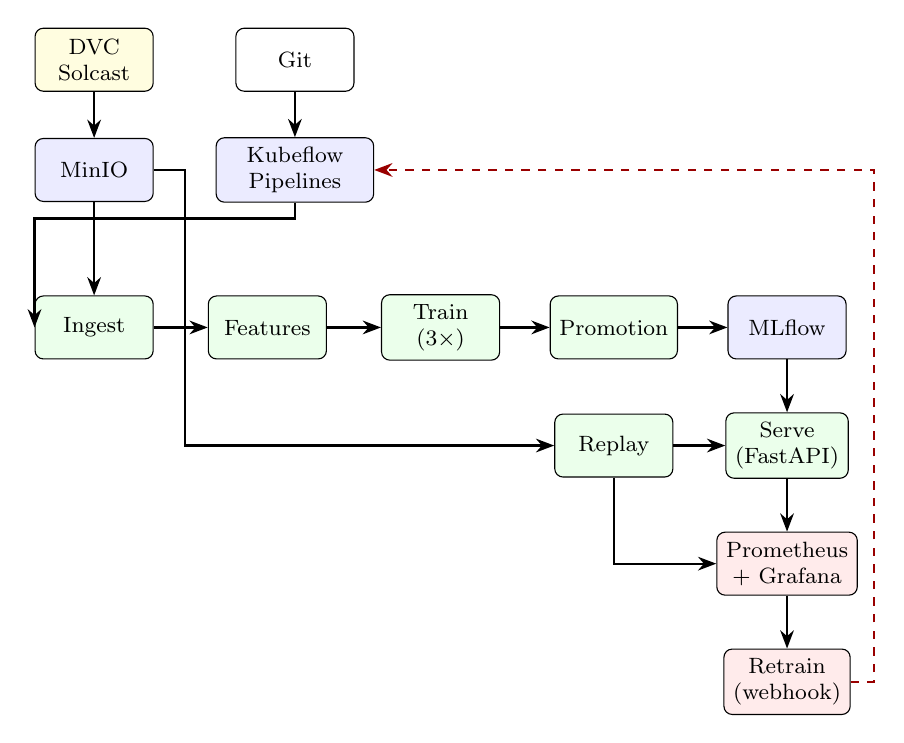
\begin{tikzpicture}[
    box/.style={rectangle, draw, rounded corners=3pt,
                minimum width=1.5cm, minimum height=0.80cm,
                align=center, font=\footnotesize},
    platform/.style={box, fill=blue!8},
    workload/.style={box, fill=green!8},
    data/.style={box, fill=yellow!12},
    monitor/.style={box, fill=red!8},
    arrow/.style={-{Stealth}, thick},
    loop/.style={-{Stealth}, thick, dashed, red!60!black},
]

% ── Row A  y=3.0 : data sources ────────────────────────────────────
\node[data]     (dvc)    at (0.75, 3.0) {DVC\\Solcast};
\node[box]      (git)    at (3.30, 3.0) {Git};

% ── Row B  y=1.6 : platform ────────────────────────────────────────
% MinIO.right=1.50  KFP.left=2.30  gap=0.80cm — no longer touching
\node[platform] (minio)  at (0.75, 1.6) {MinIO};
\node[platform, minimum width=2.0cm]
                (kfp)    at (3.30, 1.6) {Kubeflow\\Pipelines};

% ── Row C  y=-0.4 : pipeline stages ────────────────────────────────
% 1.20 cm open gap below platform for the KFP→Ingest bridge arrow
\node[workload] (ingest) at (0.75,-0.4) {Ingest};
\node[workload] (feat)   at (2.95,-0.4) {Features};
\node[workload] (train)  at (5.15,-0.4) {Train\\(3$\times$)};
\node[workload] (promo)  at (7.35,-0.4) {Promotion};
\node[platform] (mlflow) at (9.55,-0.4) {MLflow};

% ── Row D  y=-1.9 : serving ────────────────────────────────────────
\node[workload] (replay) at (7.35,-1.9) {Replay};
\node[workload] (serve)  at (9.55,-1.9) {Serve\\(FastAPI)};

% ── Row E  y=-3.4 : monitoring ─────────────────────────────────────
\node[monitor]  (kps)    at (9.55,-3.4) {Prometheus\\+ Grafana};

% ── Row F  y=-4.9 : retrain ────────────────────────────────────────
\node[monitor]  (retrain) at (9.55,-4.9) {Retrain\\(webhook)};

% ── Arrows ─────────────────────────────────────────────────────────

% Sources → Platform (straight vertical)
\draw[arrow] (dvc)   -- (minio);
\draw[arrow] (git)   -- (kfp);

% MinIO → Ingest (data): straight vertical — MinIO stores the DVC feature
%   artifacts that the Ingest stage reads.  Arrives at ingest.north.
\draw[arrow] (minio) -- (ingest);

% MinIO → Replay (data): replay.parquet read by solar-replay for drift
%   monitoring.  Steps 0.40 right of minio.east (x=1.90, in the
%   Ingest–Feat gap: Ingest.right=1.50, Feat.left=2.20), drops through
%   Row C at x=1.90, then sweeps right along y=−1.90 to replay.west.
%   Visually crosses the KFP–Ingest orchestration line at (1.90,1.00).
\draw[arrow] (minio.east) -- ++(0.40,0) |- (replay.west);

% KFP → Ingest (orchestration): step 0.20 below kfp.south (y=1.00, in
%   the 1.20cm gap), sweep left at y=1.00, drop into ingest.west.
%   Arrives at ingest.west so the two ingest arrows have separate anchors.
\draw[arrow] (kfp.south) -- ++(0,-0.20) -| (ingest.west);

% Pipeline chain (horizontal)
\draw[arrow] (ingest) -- (feat);
\draw[arrow] (feat)   -- (train);
\draw[arrow] (train)  -- (promo);
\draw[arrow] (promo)  -- (mlflow);

% MLflow → Serve (vertical)
\draw[arrow] (mlflow) -- (serve);

% Replay → Serve (horizontal)
\draw[arrow] (replay) -- (serve);

% Serve → Prometheus (vertical)
\draw[arrow] (serve) -- (kps);

% Replay → Prometheus (down to kps row, then right into kps.west)
\draw[arrow] (replay.south) |- (kps.west);

% Prometheus → Retrain (vertical)
\draw[arrow] (kps) -- (retrain);

% Retrain → KFP loop: step 0.30cm right of retrain.east (x=10.60,
%   clear of all right-column nodes whose right edge is at x=10.30),
%   then up to y=1.60, then left along Row B to kfp.east=(4.30,1.60)
\draw[loop] (retrain.east) -- ++(0.30,0) |- (kfp.east);

\end{tikzpicture}
\caption{High-level system architecture. DVC and Git feed platform services; KFP orchestrates the training pipeline; MLflow registers the best model and serves it via FastAPI; Prometheus monitors residuals and PSI, alerting a retrain webhook that triggers fresh KFP runs.}
\label{fig:architecture}
\end{figure}

The DVC-based feature engineering stage runs \emph{outside} the KFP DAG and publishes versioned artifacts to MinIO. The KFP pipeline then verifies features exist at \texttt{s3://solar-features/<git\_sha>/} before training. This deliberate separation ensures that feature computation -- which depends on external data -- is decoupled from model training, which depends only on the computed features.

% ── 3. Forecast Definition ────────────────────────────────────────────────
\section{Forecast Definition}

\begin{table}[H]
\centering
\begin{tabular}{@{}ll@{}}
\toprule
\textbf{Parameter} & \textbf{Value} \\
\midrule
Site                 & Wolf Point, MT ($48.30783^\circ$N, $105.1017^\circ$W) \\
Targets              & GHI, DNI, DHI  --  each a direct model output \\
Horizons             & 15 min (1 step) and 1 h (4 steps) \\
Outputs per call     & 6 = 3 targets $\times$ 2 horizons \\
Data resolution      & 15 minutes (Solcast historicals, UTC) \\
Baseline             & Smart persistence on the clear-sky index $k_t$ \\
Promotion rule       & Mean skill score vs. persistence on the 2-month promotion window \\ 
                     & must beat the current Production model by $\geq 0.02$ \\
\bottomrule
\end{tabular}
\caption{Forecast Configuration}
\label{tab:forecast}
\end{table}

\subsection{Split Strategy}

The data is split by timestamp -- \emph{not} by random sampling -- to preserve the temporal structure essential for time-series forecasting:

\begin{itemize}
    \item \textbf{Train:} Oldest record to $\text{reference\_now} - 8$ months
    \item \textbf{Promotion window:} $\text{reference\_now} - 8$ months to $\text{reference\_now} - 6$ months
    \item \textbf{Replay window:} Most recent 6 months (for drift monitoring)
\end{itemize}

The \texttt{reference\_now} parameter in \texttt{params.yaml} anchors all splits relative to the latest available timestamp.

\subsection{Smart Persistence Baseline}

The baseline is not naive persistence (repeating the last observed value) but \emph{smart persistence} operating on the clear-sky index $k_t$. The clear-sky index is defined as:

\begin{equation}
k_t = \frac{\text{GHI}_{\text{observed}}}{\text{GHI}_{\text{clear-sky}}}
\end{equation}

where $\text{GHI}_{\text{clear-sky}}$ is computed via the Ineichen clear-sky model parameterized for the site's latitude, longitude, altitude, and panel orientation. Persistence of $k_t$ is then converted back to physical irradiance units via the clear-sky envelope. This approach accounts for the diurnal cycle and seasonal variation that naive persistence ignores.

% ── 4. Data Pipeline ──────────────────────────────────────────────────────
\section{Data Pipeline}

\subsection{Ingestion (Stage 1)}

The raw Solcast CSV file (\texttt{data/raw/solcast.csv}) contains the following columns at 15-minute resolution, period-ending UTC:

\begin{itemize}
    \item \texttt{ghi}, \texttt{dni}, \texttt{dhi}, \texttt{gti}  --  irradiance components (W/m$^2$)
    \item \texttt{air\_temp}  --  air temperature ($^\circ$C)
    \item \texttt{wind\_speed\_100m}  --  wind speed at 100 m AGL (m/s)
    \item \texttt{zenith}, \texttt{azimuth}  --  solar geometry
\end{itemize}

The ingestion stage renames columns to canonical names, validates schemas, applies the time-based split according to \texttt{params.yaml}, and writes Parquet files to \texttt{data/interim/} along with a \texttt{splits.json} manifest.

\subsection{Feature Engineering (Stage 2)}

The feature engineering stage computes the following features from the ingested data:

\begin{itemize}
    \item \textbf{Clear-sky index} $k_t$ with clipping to $[0, 1.5]$
    \item \textbf{Lagged variables} at 15 min, 1 h, and 3 h offsets for GHI, DNI, DHI, $k_t$, air temperature, and wind speed
    \item \textbf{Rolling means} over 1 h and 3 h windows
    \item \textbf{Nighttime filtering} using a zenith angle threshold of $90^\circ$
    \item \textbf{Solar geometry features}: sine and cosine of solar hour angle, day of year encoding
\end{itemize}

The output consists of three Parquet files -- \texttt{train.parquet}, \texttt{promo.parquet}, \texttt{replay.parquet} -- plus a \texttt{features\_manifest.json} that records the schema, row counts, and the SHA of the DVC lock file.

\subsection{DVC Pipeline}

Both stages are orchestrated by DVC (\texttt{dvc.yaml}):

\begin{lstlisting}[language=bash]
dvc repro  # runs ingest → features in sequence
\end{lstlisting}

DVC tracks all dependencies (source code, parameters, raw data) and only reruns stages whose dependencies have changed. The feature artifacts are versioned and can be pushed to the MinIO remote for the KFP pipeline to consume.

% ── 5. Model Training ─────────────────────────────────────────────────────
\section{Model Training}

The KFP pipeline (\texttt{pipelines/kubeflow/pipeline.py}) defines a DAG with the following stages:

\begin{enumerate}
    \item \textbf{Ingest}  --  Verify feature artifacts exist in MinIO at the current \texttt{git\_sha}
    \item \textbf{Features}  --  Load and validate the feature tables from MinIO
    \item \textbf{Train (parallel)}  --  Three containers run simultaneously:
    \begin{itemize}
        \item \texttt{train\_persistence}  --  Computes the smart persistence baseline predictions
        \item \texttt{train\_xgb}  --  Trains 6 independent XGBoost regressors (one per target $\times$ horizon)
        \item \texttt{train\_lstm}  --  Trains a single LSTM with a 6-unit output head
    \end{itemize}
    \item \textbf{Promotion}  --  Evaluates all models on the 2-month promotion window; the model with the highest mean skill score vs. persistence that beats the current Production model by $\geq 0.02$ is registered and promoted to the \texttt{Production} stage in the MLflow model registry.
\end{enumerate}

\subsection{Model Configurations}

\begin{table}[H]
\centering
\begin{tabular}{@{}ll@{}}
\toprule
\textbf{Model} & \textbf{Configuration} \\
\midrule
\multirow{3}{*}{XGBoost} & $n_{\text{estimators}} = 500$, $\text{max\_depth} = 6$ \\
                         & $\eta = 0.05$, subsample $= 0.8$ \\
                         & colsample\_bytree $= 0.8$, early\_stopping\_rounds $= 25$ \\
\midrule
\multirow{4}{*}{LSTM}    & 1-layer unidirectional LSTM, hidden\_size $= 64$ \\
                         & Dropout $= 0.2$, batch\_size $= 256$ \\
                         & Adam optimizer, $\text{lr} = 0.001$, MSE loss \\
                         & Trained on most recent 3 years of train split \\
\midrule
\multirow{2}{*}{Cross-validation} & Rolling-origin scheme, 3 splits \\
                         & Test size: 2,880 steps (30 days), gap: 4 steps (1 h) \\
\bottomrule
\end{tabular}
\caption{Model Hyperparameters (from \texttt{params.yaml})}
\label{tab:hyperparams}
\end{table}

Rolling-origin (walk-forward) cross-validation is used rather than random k-fold to preserve the temporal order of the data. Each split trains on all history up to a cut-point, then evaluates on the next 30 days; the 1-hour gap between the train end and the test start prevents target leakage from lagged features. XGBoost and persistence train on the full $\approx$18-year train split; the LSTM is restricted to the most recent 3 years (\texttt{train\_subsample\_years: 3} in \texttt{params.yaml}), which is sufficient to cover full seasonal cycles while keeping CPU training time tractable.

\subsection{Skill Score}

The promotion metric is the skill score, defined as:

\begin{equation}
\text{Skill} = 1 - \frac{\text{RMSE}_{\text{model}}}{\text{RMSE}_{\text{persistence}}}
\end{equation}

A positive skill score indicates the model outperforms the smart persistence baseline. The promotion rule requires the mean skill score across all 6 output cells to exceed the current Production model's mean skill score by at least 0.02.

% ── 6. Results ────────────────────────────────────────────────────────────
\section{Results}

The following table shows the latest MLflow run per model type at the time of writing. All metrics are computed on the 2-month promotion window.

\begin{table}[H]
\centering
\small
\begin{tabular}{@{}llrrrr@{}}
\toprule
\textbf{Target} & \textbf{Horizon} & \textbf{Metric} & \textbf{Persistence} & \textbf{XGBoost} & \textbf{LSTM} \\
\midrule
\multirow{3}{*}{GHI} & \multirow{3}{*}{15min} & MAE   & 16.0  & 15.7  & 18.3 \\
                     &                        & RMSE  & 38.2  & 37.3  & 38.2 \\
                     &                        & SKILL &  --      & +0.026 & +0.002 \\
\cmidrule{2-6}
\multirow{3}{*}{GHI} & \multirow{3}{*}{1h}   & MAE   & 35.2  & 31.2  & 34.2 \\
                     &                        & RMSE  & 74.5  & 66.3  & 68.2 \\
                     &                        & SKILL &  --      & +0.111 & +0.086 \\
\midrule
\multirow{3}{*}{DNI} & \multirow{3}{*}{15min} & MAE   & 35.1  & 37.8  & 42.5 \\
                     &                        & RMSE  & 83.9  & 82.0  & 82.9 \\
                     &                        & SKILL &  --      & +0.023 & +0.013 \\
\cmidrule{2-6}
\multirow{3}{*}{DNI} & \multirow{3}{*}{1h}   & MAE   & 77.1  & 80.5  & 81.7 \\
                     &                        & RMSE  & 161.5 & 143.6 & 145.6 \\
                     &                        & SKILL &  --      & +0.112 & +0.100 \\
\midrule
\multirow{3}{*}{DHI} & \multirow{3}{*}{15min} & MAE   & 36.4  & 14.8  & 17.0 \\
                     &                        & RMSE  & 76.3  & 32.2  & 34.1 \\
                     &                        & SKILL &  --      & \textbf{+0.575} & +0.550 \\
\cmidrule{2-6}
\multirow{3}{*}{DHI} & \multirow{3}{*}{1h}   & MAE   & 39.2  & 26.6  & 27.6 \\
                     &                        & RMSE  & 78.2  & 50.4  & 51.1 \\
                     &                        & SKILL &  --      & \textbf{+0.354} & +0.345 \\
\bottomrule
\end{tabular}
\caption{Model Performance Comparison}
\label{tab:results}
\end{table}

\noindent\textit{Note:} MAE and RMSE are in W/m$^2$. Skill score is unitless. The persistence row has no skill column by construction, as skill is computed \emph{against} it.

\subsection{Key Findings}

\begin{enumerate}[leftmargin=*]
    \item \textbf{XGBoost beats LSTM on every cell}, and both beat persistence everywhere. XGBoost is the currently deployed (Production) model.
    
    \item \textbf{DHI shows the largest improvement over persistence:} +0.58 skill at 15 min and +0.35 at 1 h. Diffuse irradiance is the most volatile of the three targets, so persistence is weakest there and the engineered features carry the most signal.
    
    \item \textbf{GHI at 15 min is where persistence is hardest to beat:} at one step ahead, the last-observed clear-sky index is already a strong predictor, and the models only buy $\approx$0.5--2.5\% skill on top.
    
    \item \textbf{The LSTM closes much of the gap to XGBoost on the long-horizon DNI/DHI cells} but does not surpass it, suggesting that the feature engineering (lags, rolling means, clear-sky decomposition) already captures much of the temporal structure.
\end{enumerate}

% ── 7. Reproducibility ────────────────────────────────────────────────────
\section{Reproducibility}

Every promoted model in the MLflow registry carries two provenance tags:

\begin{table}[H]
\centering
\begin{tabular}{@{}ll@{}}
\toprule
\textbf{Tag} & \textbf{Identifies} \\
\midrule
\texttt{git\_commit} & Exact source code at the moment of training \\
\texttt{dvc\_hash}   & SHA-256 of the feature artifact entries in \texttt{dvc.lock} \\
\bottomrule
\end{tabular}
\caption{Provenance Tags}
\label{tab:provenance}
\end{table}

The rebuild procedure is:

\begin{lstlisting}[language=bash]
# 1. Read tags from the live Production model
# 2. git checkout <git_commit>
# 3. Rebuild the train Docker image
# 4. Verify: dvc_hash from dvc.lock matches the tag
# 5. Resubmit the KFP pipeline
\end{lstlisting}

If the \texttt{dvc\_hash} does not match, the pipeline aborts before training -- making silent drift between ``what was trained'' and ``what was claimed'' structurally impossible.

The repository also includes a \texttt{tests/} suite with unit tests (no cluster needed, $\approx$5 s) and integration tests (require MLflow + MinIO port-forwards). Pre-commit hooks enforce \texttt{ruff}, \texttt{black}, and \texttt{mypy} on every commit, ensuring that the source code checked into Git is always lint-clean.

% ── 8. Monitoring & Closed-Loop Retraining ────────────────────────────────
\section{Monitoring \& Closed-Loop Retraining}

\subsection{Serving API}

The FastAPI server exposes three endpoints:

\begin{table}[H]
\centering
\small
\begin{tabular}{@{}lll@{}}
\toprule
\textbf{Endpoint} & \textbf{Method} & \textbf{Description} \\
\midrule
\texttt{/predict} & POST & Returns 6 named floats (GHI/DNI/DHI $\times$ 15min/1h) \\
\texttt{/healthz} & GET  & 503 until Production model is loaded; used as liveness probe \\
\texttt{/metrics} & GET  & Prometheus text-format (latency, throughput, residuals, PSI) \\
\bottomrule
\end{tabular}
\caption{FastAPI Endpoint Summary}
\label{tab:endpoints}
\end{table}

The \texttt{/predict} request is polymorphic: tabular models (XGBoost, persistence) accept a single feature dict keyed by column name plus one \texttt{timestamp\_utc}; the LSTM accepts a list of $L = 24$ consecutive feature dicts (oldest first) plus a corresponding \texttt{timestamps\_utc} list. The server auto-detects the model flavour on startup and validates that the incoming shape matches.

\subsection{Metrics Pipeline}

The monitoring stack uses \textbf{kube-prometheus-stack} (Prometheus + Grafana + Alertmanager):

\begin{itemize}
    \item \texttt{solar-serve} exposes \texttt{/metrics} with prediction latency and throughput
    \item \texttt{solar-replay} streams 6 months of historical data through the serving endpoint, computing residuals, Population Stability Index (PSI), and skill score, all exposed via Prometheus metrics
    \item Grafana dashboards display live predictions, residuals, PSI, and skill score over time
\end{itemize}

\subsection{Alerting Rules}

Two Prometheus alerting rules guard the deployed model:

\begin{enumerate}
    \item \textbf{SolarDriftHigh}  --  Fires when the 10-minute moving average of PSI exceeds 3.0. The threshold is deliberately raised above the industry-standard 0.2 because the training-split reference distribution spans $\approx$18 years while the replay window covers only the most recent 6 months; this seasonal/climate asymmetry produces a baseline PSI of $\approx$1.5 at this site, so 0.2 would fire continuously on healthy traffic.
    \item \textbf{SolarSkillScoreLow}  --  Fires when the skill score vs.\ persistence drops below 0.0 (i.e., the model becomes worse than the baseline)
\end{enumerate}

When either alert fires, Alertmanager routes a webhook to \texttt{solar-retrain}, which:

\begin{enumerate}
    \item Checks a debounce timer (30-minute cooldown between retrains)
    \item Submits a new KFP pipeline run via the KFP API at the same \texttt{git\_sha} baked into its image
    \item The pipeline trains a new candidate $\rightarrow$ evaluates on the promotion window $\rightarrow$ promotes if it beats Production
\end{enumerate}

\subsection{Debounce Mechanism}

The retrain receiver uses a simple in-memory debounce with a 30-minute cooldown (\texttt{cooldown\_minutes: 30} in \texttt{params.yaml}). This prevents alert storms from triggering dozens of concurrent retrain runs. For production, a Redis-backed or CRD-backed state store would be more robust, but the single-replica in-memory approach is sufficient for a demonstration cluster.

% ── 9. Lessons Learned ───────────────────────────────────────────────────
\section{Lessons Learned}

\subsection{kube-prometheus-stack Defaults Silently Drop Unlabeled Alerts}

When the retrain webhook was first wired up, alerts fired in Prometheus and landed in Alertmanager -- but never reached the receiver. The root cause was the default \texttt{alertmanagerConfigMatcherStrategy: OnNamespace} on the Alertmanager CR: it auto-injects a \texttt{namespace} label matcher onto every sub-route generated from an \texttt{AlertmanagerConfig}. Prometheus does \emph{not} auto-add a \texttt{namespace} label to alerts produced by \texttt{PrometheusRule} CRs, so the match fails silently. The fix was to set \texttt{namespace: monitoring} explicitly on every alert's labels block.

\subsection{Memory Constraints on 12 GB minikube}

The \texttt{make e2e} flow assumes headroom for \texttt{serve + replay + monitoring + 3 $\times$ training pods} in parallel. At 12 GB, the LSTM and XGBoost pods compete for memory during the training stage, and one of them is OOM-killed roughly 1 time in 3 when other workloads are concurrently active. Mitigations included ordering replay \emph{after} the pipeline finishes and bumping the cluster default from 7.2 GB to 12 GB.

\subsection{DVC--KFP Separation is Intentional but Manual}

Feature engineering (\texttt{dvc repro}) runs outside the KFP DAG by design, publishing versioned artifacts to MinIO. The KFP pipeline then verifies features exist at \texttt{s3://solar-features/<git\_sha>/} before training. When an ad-hoc retrain was triggered for a SHA whose features had not been published, the pipeline failed with a 404 on \texttt{train.parquet}. The Makefile resolves this via dependency chaining (\texttt{features $\rightarrow$ pipeline}), but ad-hoc retrain triggers still require operator awareness.

\subsection{Receiver-Side Image Management}

The retrain receiver bakes its \texttt{GIT\_SHA} at build time and submits the training pipeline at the same SHA. This guarantees provenance but means that building a new \texttt{solar-retrain:<sha>} image also requires a matching \texttt{solar-train:<sha>} already loaded in minikube. The \texttt{make build} target builds all four images at the same SHA, making the e2e flow hermetic.

\subsection{LSTM Early Stopping Does Not Automatically Restore Best Weights}

PyTorch's training loop does not implicitly roll back to the best checkpoint when early stopping triggers. Without an explicit \texttt{copy.deepcopy} of the model state at each skill improvement, the artifact uploaded to MLflow reflects the \emph{last} training epoch rather than the \emph{best} one. Because early stopping fires after \texttt{patience} epochs without improvement, the saved weights may be several epochs past the model's peak validation skill. The fix is to deepcopy the state dict whenever the best skill improves, then call \texttt{load\_state\_dict} to restore it before promotion scoring and artifact upload.

% ── 10. Limitations & Future Work ──────────────────────────────────────────
\section{Limitations \& Future Work}

\begin{table}[H]
\centering
\small
\begin{tabular}{@{}p{4cm}p{8cm}@{}}
\toprule
\textbf{Limitation} & \textbf{Future Direction} \\
\midrule
In-memory debounce on retrain webhook & Redis-backed or CRD-backed state store; move debounce into Alertmanager's \texttt{repeat\_interval} \\
\midrule
6-output models trained as one multi-output head & Shared trunk + per-output heads; could lift harder cells (especially DNI) \\
\midrule
Retrain trigger fires on threshold, not trend & Trend-based detection (e.g., Mann-Kendall test on rolling PSI) for slow-drifting features \\
\midrule
One physical site, fixed orientation & Generalize to N sites via per-site \texttt{Location} objects and site-aware features \\
\midrule
LSTM weight init is the only non-determinism & \texttt{torch.manual\_seed} is pinned; GPU cuDNN nondeterminism would need additional handling \\
\midrule
No HPA on serving Deployment & Single-replica deployment; HPA not needed for demo-scale traffic \\
\midrule
No CI/CD integration & Push-to-GitHub-triggered CI workflow for automatic feature publishing and pipeline submission \\
\bottomrule
\end{tabular}
\caption{Limitations and Future Directions}
\label{tab:limitations}
\end{table}

% ── 11. Conclusion ────────────────────────────────────────────────────────
\section{Conclusion}

This project demonstrates a complete, reproducible MLOps pipeline for short-term solar irradiance forecasting. The system covers the full lifecycle: data versioning (DVC), feature engineering, multi-model training (persistence + XGBoost + LSTM), model promotion by skill score, FastAPI serving on Kubernetes, Prometheus-based monitoring with drift and skill alerts, and closed-loop retraining via Kubeflow Pipelines.

The XGBoost model achieves the best overall performance, with skill scores of up to +0.58 over the smart persistence baseline on the most challenging target (DHI). Every artifact in the system is traceable to its exact source code (Git commit) and feature input (DVC hash), ensuring full reproducibility. The end-to-end demo runs in under an hour on a local minikube cluster with 12 GB of RAM.

The key lessons -- silent alert dropping in kube-prometheus-stack, memory pressure on constrained clusters, the deliberate DVC--KFP separation, and the need to explicitly checkpoint best-epoch weights in PyTorch early stopping -- highlight the practical challenges of building production-grade MLOps systems and provide guidance for future projects.

% ── Appendix ──────────────────────────────────────────────────────────────
\appendix
\section{Quick Start}

\begin{lstlisting}[language=bash]
# Bring up the cluster and platform services (~10 min)
make cluster-up && make platform

# Run the full end-to-end demo (~45-60 min on a fresh cluster)
make e2e
\end{lstlisting}

When \texttt{make e2e} completes, open the dashboards:

\begin{lstlisting}[language=bash]
make ports
# MLflow:5000  KFP:8080  Grafana:3000  Prometheus:9090  MinIO:9001
\end{lstlisting}

\noindent The \texttt{make e2e} target chains: \texttt{build → features → pipeline → serve → monitoring → retrain → replay → trigger-drift → verify}.

\end{document}
